\documentclass[../main.tex]{subfiles}
\graphicspath{{\subfix{../img/}}}

\begin{document}

\subsection{Oscillations after \glsentrytext{ttx} Application}

\noindent It was illustrated in Section \ref{subsubsec:experiment_ttx_t_type_block} that R5 neurons exhibited slow oscillations, potentially mediated by Ca$^{2+}$ channels after the sodium channels were blocked by application of \gls{ttx}. These oscillations showed three main features: apparent \gls{ahp} (undershoot of the membrane potential below steady state), a spike with a width of approximately $\sim 100$ms, and a relatively long interspike interval on the order of seconds.
Furthermore, no oscillations were present in $Ca$-$\alpha 1T$-KD animals after blockade of sodium channels.

As discussed in Section \ref{subsec:math_backg_ttx_oscillations}, slow oscillations require either a slow timescale or the trajectory passing near the equilibrium of the full dynamical system. However, the latter scenario is generally not robust to parameter perturbations.

Out of four parameter regimes tested across three models labelled as Wang, Goldman, and Park (see Section \ref{sec:materials_and_methods} and Appendix \ref{appendix:functions_and_parameters}), only three showed oscillations with apparent \gls{ahp} - Wang \parencite{wangMultipleDynamicalModes1994} and both parameter sets of the Goldman \parencite{goldmanGlobalStructureRobustness2001} (for the latter parameters were taken from \parencite{franciRobustTunableBursting2018}). \textcolor{red}{Plot examples of voltage traces}. Neither model included gating mechanisms operating on timescales of seconds (see Appendix \ref{appendix:functions_and_parameters} for more details). 

To investigate oscillations following sodium channel blockade in adapted neuronal models, several factors were considered. First, as it was discussed in Section \ref{sec:sleep_and_r5_network}, knockdown of the T-type channels may have been partial rather than complete. Second, blockade of $Na^+$ channels does not necessarily eliminate external input to the neuron. Apart from chemical synapses, neurons may receive external input via other mechanisms, such as gap-junctions or passive leak channels. As external effects can slightly vary across individuals, minor perturbations in parameters, as well as external input, should not affect the dynamics.
Therefore, in the adapted neuronal models, all parameters were kept as specified in Section \ref{appendix:functions_and_parameters}, except for the maximal conductance of T-type channels (to account for the partial blockade) and the external input current. The spike period and width were calculated as described in Section \ref{sec:materials_and_methods}.

\begin{figure}[!t]
    \centering
    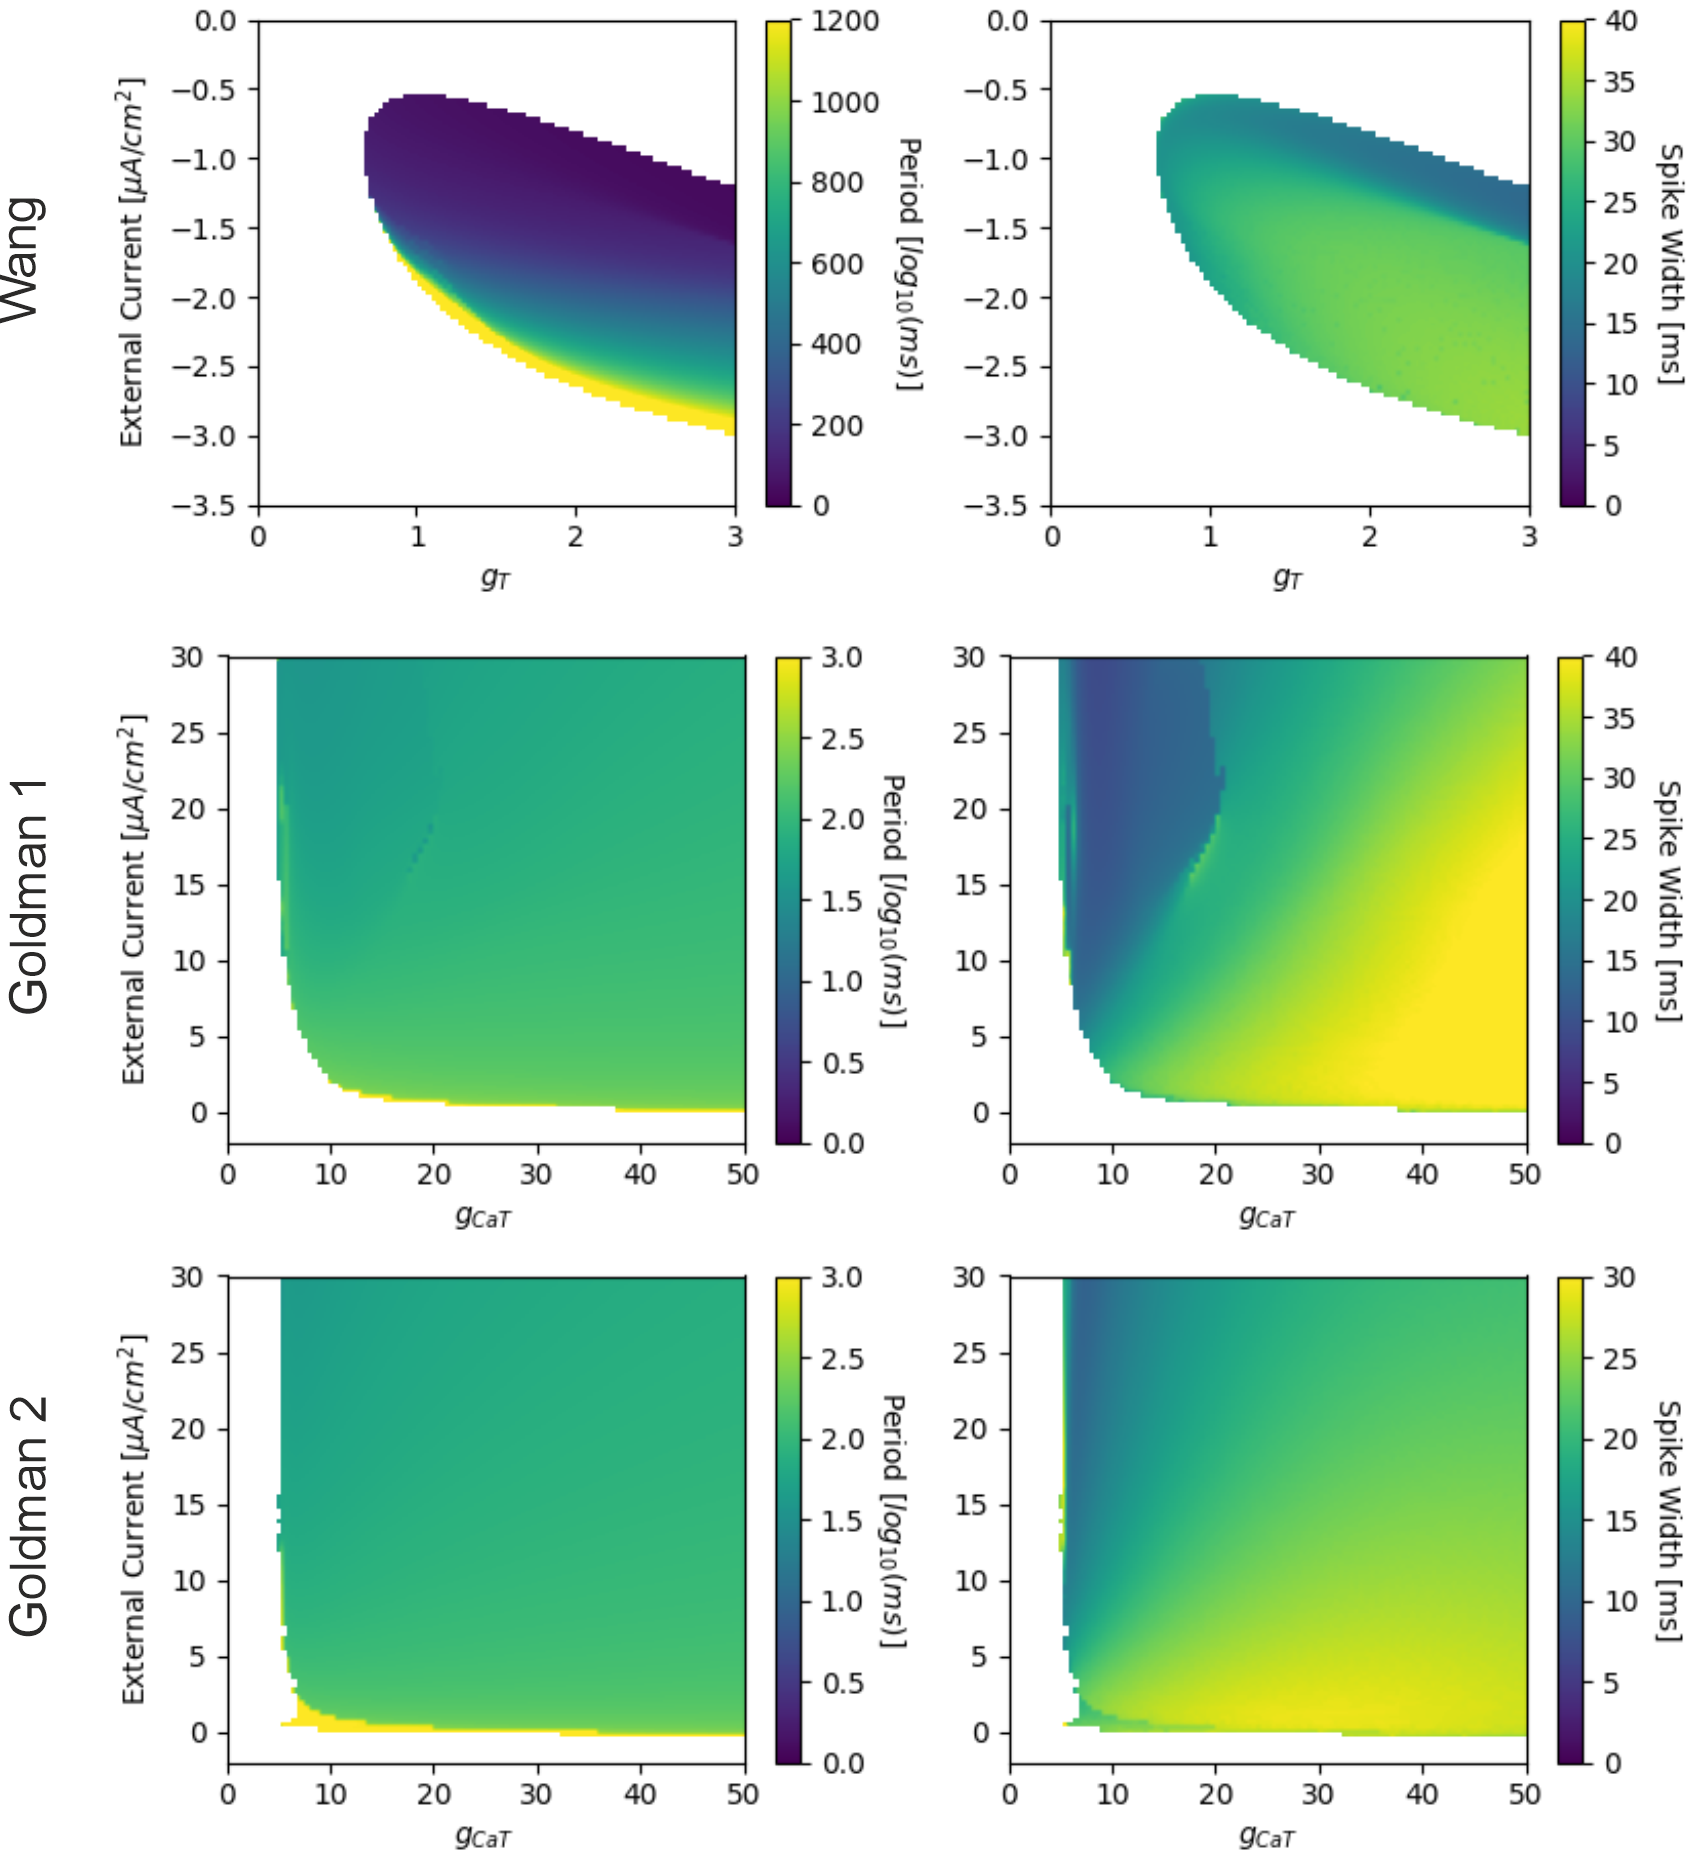
\includegraphics[width=0.9\linewidth]{../img/ttx_block/ttx_block.png}
    \caption[Effect of External Current and T-Type Conductance on Calcium Spike Width and Period]{
        \textbf{Effect of External Current and T-Type Conductance on Calcium Spike Width and Period.} \textcolor{red}{TEXT!!!. Colorbar label of the Wang is wrong, should be ms instead of log10(ms)!! Outline parts with >= 1sec period + units on x axis}
    }
    \label{fig:models_ttx_block}
\end{figure}

Figure \ref{fig:models_ttx_block} illustrates how the period and the width of the spikes depend on the conductance of T-type channels and external input current. Note that for each model, the label for the $x$ axis was chosen to be the same as described in the corresponding papers ($g_T$ and $g_{CaT}$), although they all account for the T-type Ca$^{2+}$ channel. The colored areas indicate parameter combinations where the neuron exhibited spiking activity, with the colour scale representing either period (left column) or spike width (right column). White regions correspond to the parameter values where the system did not exhibit spiking activity and converged to a resting state. In all three models, the slow oscillations ($\geq$ $1$ Hz) were confined to a narrow region of parameter space, close to the bifurcation that separates spiking and resting regimes.

Thus, the results are consistent with the predictions outlined in Section \ref{subsec:math_backg_ttx_oscillations}, and support the notion that the system requires an intrinsic slow variable to generate robust low-frequency oscillations. As discussed in Section \ref{subsubsec:experiment_ttx_t_type_block}, a potential underlying slow mechanism may be the slow removal of intracellular calcium following a spike, which could lead to the gradual inactivation of calcium-activated potassium channels. This, in turn, may contribute to the slow depolarization of the membrane potential between spikes (see also \textit{Slow-frequency oscillations following $Na^{+}$ channel blockade} in Section \ref{sec:discussion}).


\end{document}